\section{Design}
\label{sec:design}
We now discuss the design philosophy behind sybilhunter, our Sybil detection
tool.  Sybilhunter takes as input archived Tor network data, and then attempts
to isolate Sybil groups.  The big picture is shown in Figure~\ref{fig:system}.
We motivate our design decisions with the experience we gained by manually
analyzing numerous Sybil groups in the Tor network.  We iteratively improved
and refactored sybilhunter when we experienced operational shortcomings.  We
further augment our design with ideas from related work, e.g., Cao et al.
observed that Sybil groups have things in common and changes happen more or
less at the same time~\cite{Cao2014a}.

\begin{figure}[t]
	\centering
	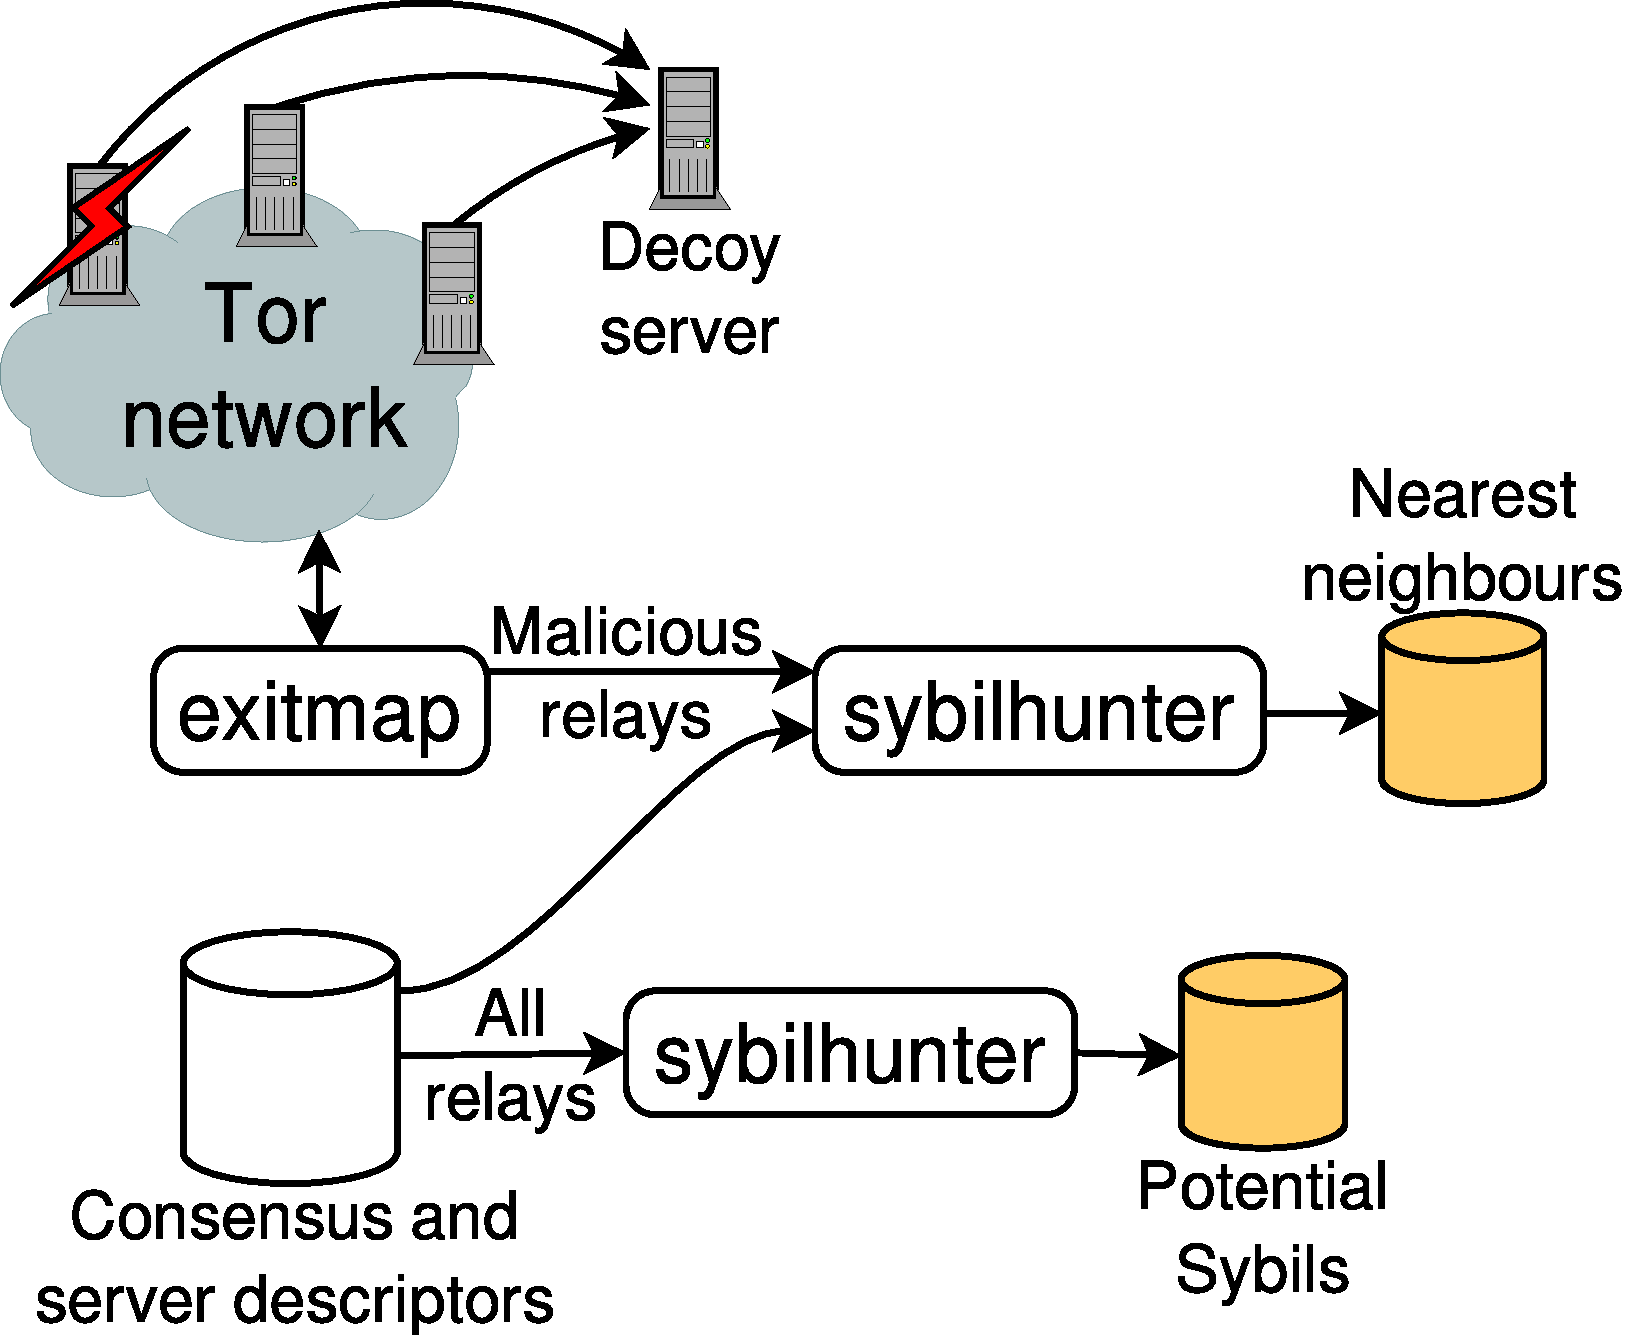
\includegraphics[width=0.42\textwidth]{diagrams/system_architecture.pdf}
	\caption{Our system architecture.  Two different data sets serve as input
		to sybilhunter, our Sybil detection tool; 1) archived consensuses and
		server descriptors, and 2) malicious relays that we gather by running
		exitmap~\cite{Winter2014a}.  Sybilhunter then attempts to extract Sybil
		groups from the given data.}
	\label{fig:system}
\end{figure}

Sybilhunter is designed to run in different scenarios.  We can 1) run it over
historical network data, ranging back to 2007, 2) run it online to detect new
Sybils as they join the network, and 3) use it to find relays that are
potentially associated with previously discovered bad exit relays.

Generally speaking, we seek to isolate relays that are similar in
\emph{appearance} as well as in \emph{behavior}.  The following sections
discuss our data sets and analysis modules of sybilhunter.

\subsection{Data sets}
We employ two types of data sets, both of which are illustrated in
Figure~\ref{fig:system}.  First, we mine \emph{archived consensuses and server
descriptors} for relay clusters and second, we use the \emph{output of the
exitmap scanner} (in combination with archived data) to find associated,
malicious relays.

\subsubsection{Consensuses and router descriptors}
We took the data sets we use for our analyses from CollecTor~\cite{collector},
a service run by The Tor Project that archives network data such as
consensuses, router descriptors, and network status votes.  Some of the
archived data dates back to as early as 2004, allowing us to restore arbitrary
Tor network states in the last ten years.  CollecTor archives numerous data
sources, but not all are relevant for our hunt for Sybils, which is why we only
analyse the following two:

\begin{description}
	\item[Descriptors] Tor relays and bridges periodically upload server
		descriptors, which capture their configuration, to directory
		authorities.  Relays upload their descriptors no later than every 18
		hours, or sooner, depending on certain conditions.

	\item[Consensuses] The Tor network's consensus contains a list of all
		running Tor relays.  Directory authorities vote hourly on the state of
		the network, and the outcome is the consensus.  Every relay status in
		the consensus contains a digest that is used to obtain the relay's
		respective descriptor, as can be seen in Figure~\ref{fig:datasets}.
\end{description}

\begin{figure}[t]
	\centering
	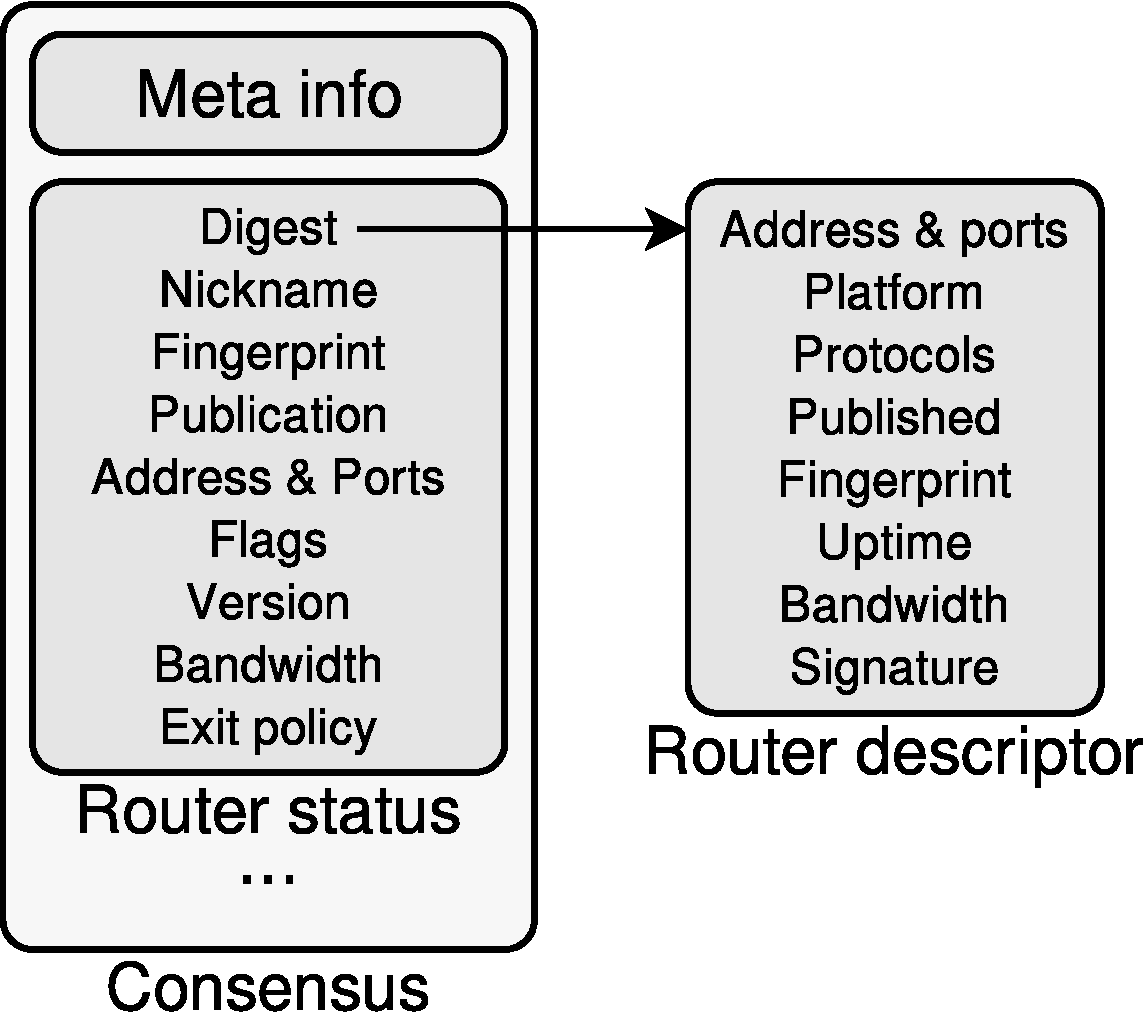
\includegraphics[width=0.3\textwidth]{diagrams/data_sets.pdf}
	\caption{Our data set contains consensuses and router descriptors.  This
		diagram shows how they relate to each other.}
	\label{fig:datasets}
\end{figure}

Table~\ref{tab:datasets} gives an overview of the size of our data sets.  We
found it challenging to process such large amounts of data.  We started by
using the Python parsing library Stem, which is maintained by The Tor Project.
The size of the data sets as well as the amount of files turned out to be
difficult to handle for Stem because it was implemented in an interpreted,
dynamic language.

\begin{table}[t]
\centering
\begin{tabular}{l c c c}
\textbf{Data set} & \textbf{Files} & \textbf{Size} & \textbf{Time span} \\
\hline
% 47677982862 bytes.
Consensuses & 67,671 & 44 GiB & 10/2007 -- 07/2015 \\
% 48252370463 bytes.
Descriptors & 30,759,243 & 44 GiB & 12/2005 -- 07/2015 \\
% 1375933490 bytes.
% Torperf data & 18,348 & 1 GiB & 07/2009 -- 07/2015 \\
\end{tabular}
\caption{Characterization of our data sets.}
\label{tab:datasets}
\end{table}

We then implemented a new parser from scratch in the Go programming
language~\cite{zoossh}.  Our parser consists of approximately 2,000 lines of
code (and 1,000 more lines for tests) and supports strict and lazy parsing, to
minimize unnecessary parsing.  According to our benchmarks, our parser is able
to parse approximately 27 consensuses per second.\footnote{Measured on an Intel
Core i7 2.9 GHz CPU.  We placed our data sets on a solid state drive to
minimize I/O.}  Stem, for comparison, averages at around 1.8 consensuses per
second.\footnote{Note, however, that Stem parses slightly more fields than our
parser, which means that both parsers would be closer together in a fair
comparison.}

Figure~\ref{fig:datasets} illustrates the relationship between our data.
Primarily, we are interested in the hourly consensus files.  A consensus file
consists of \emph{router statuses} that contain basic information about Tor
relays such as its bandwidth, flags, and exit policy.  As of August 2015,
consensuses contain approximately 6,000 router statuses.  Every router status
contains a digest that is used to locate its corresponding \emph{router
descriptor}.  It is important to understand that router descriptors are
published as they were received by Tor relays whereas consensus files are voted
on, and published, by directory authorities.  Some fields in a router status
are also subject to verification.  For example, the Tor network operates
bandwidth scanners that verify if a relay is able to sustain the bandwidth it
claims to handle in its router descriptor.

\subsubsection{Malicious relays}
We use a second, complementary data set that consists of malicious exit relays
we gather by running exitmap~\cite[\S 3.1]{Winter2014a}.  Exitmap is a
Python-based scanning framework for Tor exit relays.  Exitmap modules perform a
network task that can then be run over all exit relays.  One use case is HTTPS
MitM detection: A module can fetch the X.509 certificate of a web server over
all exit relays and then compare the fingerprint to the expected, valid
fingerprint.  In addition to the original modules, exitmap's authors shared
with us, we implemented modules to detect HTML tampering and TLS downgrading.
Our modules ran from August 2014 to August 2015 and discovered 225 malicious
exit relays, which we all reported to The Tor Project.
% blockchain.info tampering
% <20140811014615.GB23748@nymity.ch> 1
% <20140920132357.GC8751@nymity.ch> 1
% <20141021133016.GA11247@nymity.ch> 2
% <20141025182433.GA23244@nymity.ch> 1
% <20150109195428.GA29115@nymity.ch> 23
% <20150210154109.GD10777@nymity.ch> 1
% <20150804202838.GA4774@nymity.ch> 4
% <20150630022923.GA2340@nymity.ch> 55
% <20150605120807.GA20320@nymity.ch> 49
% <20150423004031.GA11395@nymity.ch> 70
% <20150311131506.GE23215@nymity.ch> 18

We include malicious exit relays in our data set because we found that they
frequently \emph{surface in groups}, i.e., an attacker runs the same attack on
several, physically distinct exit relays.  Winter et al.'s work~\cite[\S
5.2]{Winter2014a} showed that attackers make an effort to stay under the radar,
which is why we cannot only rely on active probing to find and block such
relays.  We also seek to find the \emph{nearest neighbors} of each newly
discovered malicious relay, which we discuss in
Section~\ref{sec:nearest-neighbor}.

\subsection{Threat model}
\label{sec:threat_model}
\mynote{Threat model is vague.  Ideas for better phrasing?}

Sybilhunter, our Sybil detection tool, can process \emph{past data} just as
\emph{future data}.  Future data, however, can be manipulated by adversaries
that seek to evade our system and the powerful nature of Sybil
attacks~\cite{Douceur2002a} limits us in what we can defend against.  This is
reflected in our adversarial assumptions, which we now discuss.  We expect that
an an adversary \emph{does}:
\begin{itemize}
	\item Run multiple Tor relays.

	\item Add Tor relays all at once or slowly over time.

	\item Run active or passive attacks.

	\item Make a limited effort to stay under the radar by diversifying
		different aspects of their Tor relays.
\end{itemize}

We expect that an adversary \emph{does not}:
\begin{itemize}
	\item Have infinite resources to create undetectable Sybils.
\end{itemize}

\subsection{Churn analysis}
An unexpectedly high churn rate (i.e., the rate of relays joining and leaving
the network) between two subsequent consensuses can reveal Sybils because Sybil
operators frequently start and stop their Sybils at the same time.  The Tor
Project is already running a script~\cite{doctor} that checks new consensus
documents and counts the number of relay fingerprints that have never been seen
before.  If this number exceeds 49, an alert is raised.  We reimplemented the
script in sybilhunter and ran it over all archived consensus documents, dating
back to 2007.  The script raised 47 alerts (over nine years), all of which
seemed true positives.  We will now improve on this script.

\mynote{Should add a diagram here, illustrating these two types of churn.}

We found that churn values worthy of our attention typically manifest in two
ways: \emph{sudden bursts}, as well as less sudden ``hills.'' The former can
happen if an attacker injects several dozen relays at the same time, while the
latter happened shortly after the heartbleed vulnerability; relay operators
were told to generate new keys, which didn't happen at the exact same time, but
over two days.  We use a formula proposed by Godfrey et al.~\cite{Godfrey2006a}
to determine the churn rate $\sigma$ over time.  $C_{t}$ is the network
consensus at time $t$, and $\ominus$ is the symmetric difference between two
consensuses:

$$
\sigma = \frac{1}{2} \cdot \frac{\lvert C_{t-1} \ominus C_{t} \rvert}
{\textrm{max}\{\lvert C_{t-1} \rvert, \lvert C_{t} \rvert \}}.
$$

Determining $\lambda$ for the sequence $C_{t}, C_{t+1}$, $C_{t+1}, C_{t+2}$,
etc. yields a time series.  We calculate the moving average $\lambda$ for the
time series using the following equation:

$$
\lambda = \frac{1}{w} \cdot \sum_{n=0}^{w} \sigma_{n}.
$$

We found that a window size $w$ covering several hours brings the best results.
In an operating setting, we believe that this parameter should be kept secret
as it would help attackers to stay under the radar.  Refer to
Section~\ref{sec:secrecy} for a more comprehensive discussion.  If $\lambda$
exceeds a manually defined threshold, an alert is raised.

\subsection{Fingerprint analysis}
The information a Tor client needs to connect to a hidden service is saved in a
distributed hash table (DHT) that consists of a subset of all Tor relays, the
so called hidden service directories (HSDirs).  A daily changing set of six
HSDirs are responsible for a hidden service, i.e., clients ask them for
information about the hidden service they want to connect to.

A HSDir becomes responsible for a hidden service based on its fingerprint.
Note that the DHT and all its HSDirs is known and it is also possible to
calculate which index in the fingerprint ring will be used by a hidden service
at a future point in time~\cite{Biryukov2013a}.  Attackers can exploit this
knowledge by generating identity keys until their fingerprint is close to the
hidden service's index, thus becoming responsible for it.  To save resources,
an attacker can run a single, physical Tor relay and generate a new identity
periodically.

We seek to detect relays that change their fingerprint frequently by building a
table that maps a relay's IP addresses to all the fingerprints we have observed
for it.

\subsection{Uptime analysis}
An attacker is likely to administer her Sybils in parallel, i.e., start and
stop them at approximately the same time.  We exploit this fact by comparing
the \emph{uptime patterns} of Tor relays.  Relays with a similar uptime pattern
are more likely to be under common administrative control than the same relays
with a differing uptime pattern.

We represent the uptime pattern as a binary sequence.  Every hour, when a new
consensus is published, we extend the sequence with a new data point for each
Tor relay.  It is tempting to use the Hamming distance to quantify the
similarity between two relays.  The Hamming distance is the amount of positions
at which two strings of equal length differ.  This, however, does not perfectly
capture our intuition as we show in Figure~\ref{fig:uptime-pattern}.  Relay $B$
and $C$ have the same Hamming distance with relay $A$: two.  Intuitively,
however, we consider relay $B$ to be more similar to relay $A$ than is $C$
because it does not exhibit the uptime sequence at hour seven and eight.  We
consider this by increasing a \emph{deviation amplifier} as two uptime sequences
continue to diverge (see Algorithm~\ref{alg:uptime}).  As long as two sequences
keep deviating, our deviation amplifier is increased by 0.1 until it reaches 1.  As
soon as two sequences converge again, the deviation error is reset to 0.
Finally, we divide the distance by the sequence length to normalize it to the
interval $[0, 1]$.

According to this algorithm, relay $A$ and $B$ in
Figure~\ref{fig:uptime-pattern} have a similarity of 0.1 + 0.1 while $A$ and
$C$ have a similarity of 0.1 + 0.2.

\begin{figure}[t]
\centering
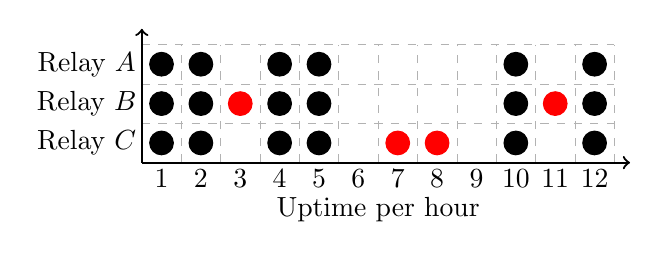
\begin{tikzpicture}
\draw[help lines, color=gray!60, dashed, step=0.5] (0,0) grid (6,1.5);
\draw[->,thick] (0,0)--(6.2,0);% node[midway, below]{Uptime per hour};
%node [midway, fill=white, text centered]
%\put(4,1){test};
%\put(4,0.5){\makebox(0,1)[b]{foo}}
%node[below left]{$x$};
\draw[->,thick] (0,0)--(0,1.7);% node[midway, above, rotate=90]{Relay ID};

% Y labels.
\node at (-0.7,1.25) {Relay $A$};
\node at (-0.7,0.75) {Relay $B$};
\node at (-0.7,0.25) {Relay $C$};

% X labels.
\node at (0.25, -0.2) {1};
\node at (0.75, -0.2) {2};
\node at (1.25, -0.2) {3};
\node at (1.75, -0.2) {4};
\node at (2.25, -0.2) {5};
\node at (2.75, -0.2) {6};
\node at (3.25, -0.2) {7};
\node at (3.75, -0.2) {8};
\node at (4.25, -0.2) {9};
\node at (4.75, -0.2) {10};
\node at (5.25, -0.2) {11};
\node at (5.75, -0.2) {12};

\node at (3, -0.6) {Uptime per hour};

% Relay A.
\filldraw[black] (0.25,1.25) circle (0.15);
\filldraw[black] (0.75,1.25) circle (0.15);

\filldraw[black] (1.75,1.25) circle (0.15);
\filldraw[black] (2.25,1.25) circle (0.15);

\filldraw[black] (4.75,1.25) circle (0.15);

\filldraw[black] (5.75,1.25) circle (0.15);

% Relay B.
\filldraw[black] (0.25,0.75) circle (0.15);
\filldraw[black] (0.75,0.75) circle (0.15);
\filldraw[red]   (1.25,0.75) circle (0.15);
\filldraw[black] (1.75,0.75) circle (0.15);
\filldraw[black] (2.25,0.75) circle (0.15);

\filldraw[black] (4.75,0.75) circle (0.15);
\filldraw[red]   (5.25,0.75) circle (0.15);
\filldraw[black] (5.75,0.75) circle (0.15);

% Relay C.
\filldraw[black] (0.25,0.25) circle (0.15);
\filldraw[black] (0.75,0.25) circle (0.15);

\filldraw[black] (1.75,0.25) circle (0.15);
\filldraw[black] (2.25,0.25) circle (0.15);

\filldraw[red]   (3.25,0.25) circle (0.15);
\filldraw[red]   (3.75,0.25) circle (0.15);

\filldraw[black] (4.75,0.25) circle (0.15);

\filldraw[black] (5.75,0.25) circle (0.15);
\end{tikzpicture}

\caption{Uptime pattern of three relays.  Intuitively, relay $B$ is more
similar to relay $A$ than is relay $C$, but the Hamming distance is two for
both patterns.}
\label{fig:uptime-pattern}
\end{figure}

\begin{algorithm}[t]
\caption{Our algorithm to quantify the similarity between the uptime pattern
of two relays $A$ and $B$.}
\label{alg:uptime}
\begin{algorithmic}[1]
\Function{Distance}{$A, B$}
    \State $dist \gets 0$
    \State $amp \gets 0$

    \For{$t$ \textbf{in} $hours$}
        \If{$A_{t} \ne B_{t}$}
            \If{$amp < 1$}
                \State $amp \gets amp + 0.1$
            \EndIf
        \State $dist \gets dist + amp$
        \Else
            \State $amp \gets 0$
        \EndIf
    \EndFor
    \State \textbf{return} $dist / \lvert hours \rvert$
\EndFunction
\end{algorithmic}
\end{algorithm}

\subsection{Nearest-neighbor search}
\label{sec:nearest-neighbor}
We frequently found ourselves in a situation where exitmap discovered a
malicious exit relay and we were trying to find similar, potentially associated
relays.  This involved extensive manual work, which we soon started to
automate.  We needed an algorithm for nearest-neighbor search: given a
reference relay, what are its $n$ nearest neighbors?

A naive implementation would compare the reference relay to all other relays in
the consensus, which scales linearly.  We can do better by using metric trees,
which guarantee $\mathcal{O}(\textrm{log} n)$ lookup.  Metric trees are a type
of data structure to index data in metric spaces, and need a distance metric in
the mathematical sense.  A mathematical metric requires a number of conditions
to be met (see Appendix~\ref{sec:metric}), which are not always satisfied by
ad-hoc metrics.  In particular, the triangle inequality\footnote{The triangle
inequality, $d(x, z) \le d(x, y) + d(y, z)$, states that the distance between
two points is at least equal to a ``detour'' over a third point.} can be
difficult to meet when working in non-Euclidean space.

We use the Levenshtein distance as distance metric.  It determines the minimum
amount of modifications---insert, delete, and modify---that are necessary to
turn string $s_{1}$ into $s_{2}$.  The Levenshtein distance can handle strings
of different length, and satisfies the triangle inequality, which means that we
are free to use it in a metric tree.

As concrete variant of our metric tree, we use a the vantage point tree
(vp-tree)~\cite{Yianilos1993a}.  It recursively divides the given data into two
partitions: one that is close to the reference point according to a threshold,
and one that is not.  The vp-tree must first be built.
%which takes $\mathcal{O}()$ operations.
It is then ready to perform nearest neighbor
searches.

In our implementation, building a vp-tree for 6,235 relays takes approximately
10 seconds.\footnote{Again, measured on an Intel Core i7 2.9 GHz CPU.}
Subsequent nearest-neighbor lookups finish almost instantly.

\mynote{Still need to compare this to naive $n^{2}$ search.}

\subsection{Blocking Sybils}
Once we isolated a Sybil group, and concluded that it appears to be harmful, we
reported it to The Tor Project.  There are currently two ways for directory
authorities to block relays, controlled by the options \texttt{AuthDirReject}
and \texttt{AuthDirInvalid}.  The former removes a relay from the consensus.
The latter takes away a relay's \texttt{Valid} flag.  While the relay is still
listed in the consensus, clients will not consider it for path selection.

The majority of directory authorities, i.e., five out of nine, must agree on
either \texttt{AuthDirReject} or \texttt{AuthDirInvalid} be set for a relay.
Only then will the block become active.  This is done to distribute the power
of removing relays into the hands of a diverse set of people.  We elaborate on
our experience with this process in Section~\ref{sec:operational}.

\subsection{Meaningful results}
Systems that employ complex and opaque analysis techniques to expose security
incidents frequently suffer from what Sommer and Paxson call the \emph{semantic
gap}~\cite[\S III.C]{Sommer2010a}, i.e., a system's output is difficult to act
upon as its meaning is unclear.  Our tools automate the detection of Sybils,
but the process of blocking them involves human interaction, which is why we
took special care to consider the semantic gap.

First, we avoid the use of opaque classification models as their output (often
distances in high-dimensional vector space) is difficult to comprehend.
Instead, we use simple string metrics such as the Levenshtein distance.
Figure~\ref{fig:visualization} illustrates a visualization we developed for
exploratory analysis that can complement automated analysis.  The graph shows
the similarities (edges) between four Tor relays (vertices).

\begin{figure}[t]
	\centering
	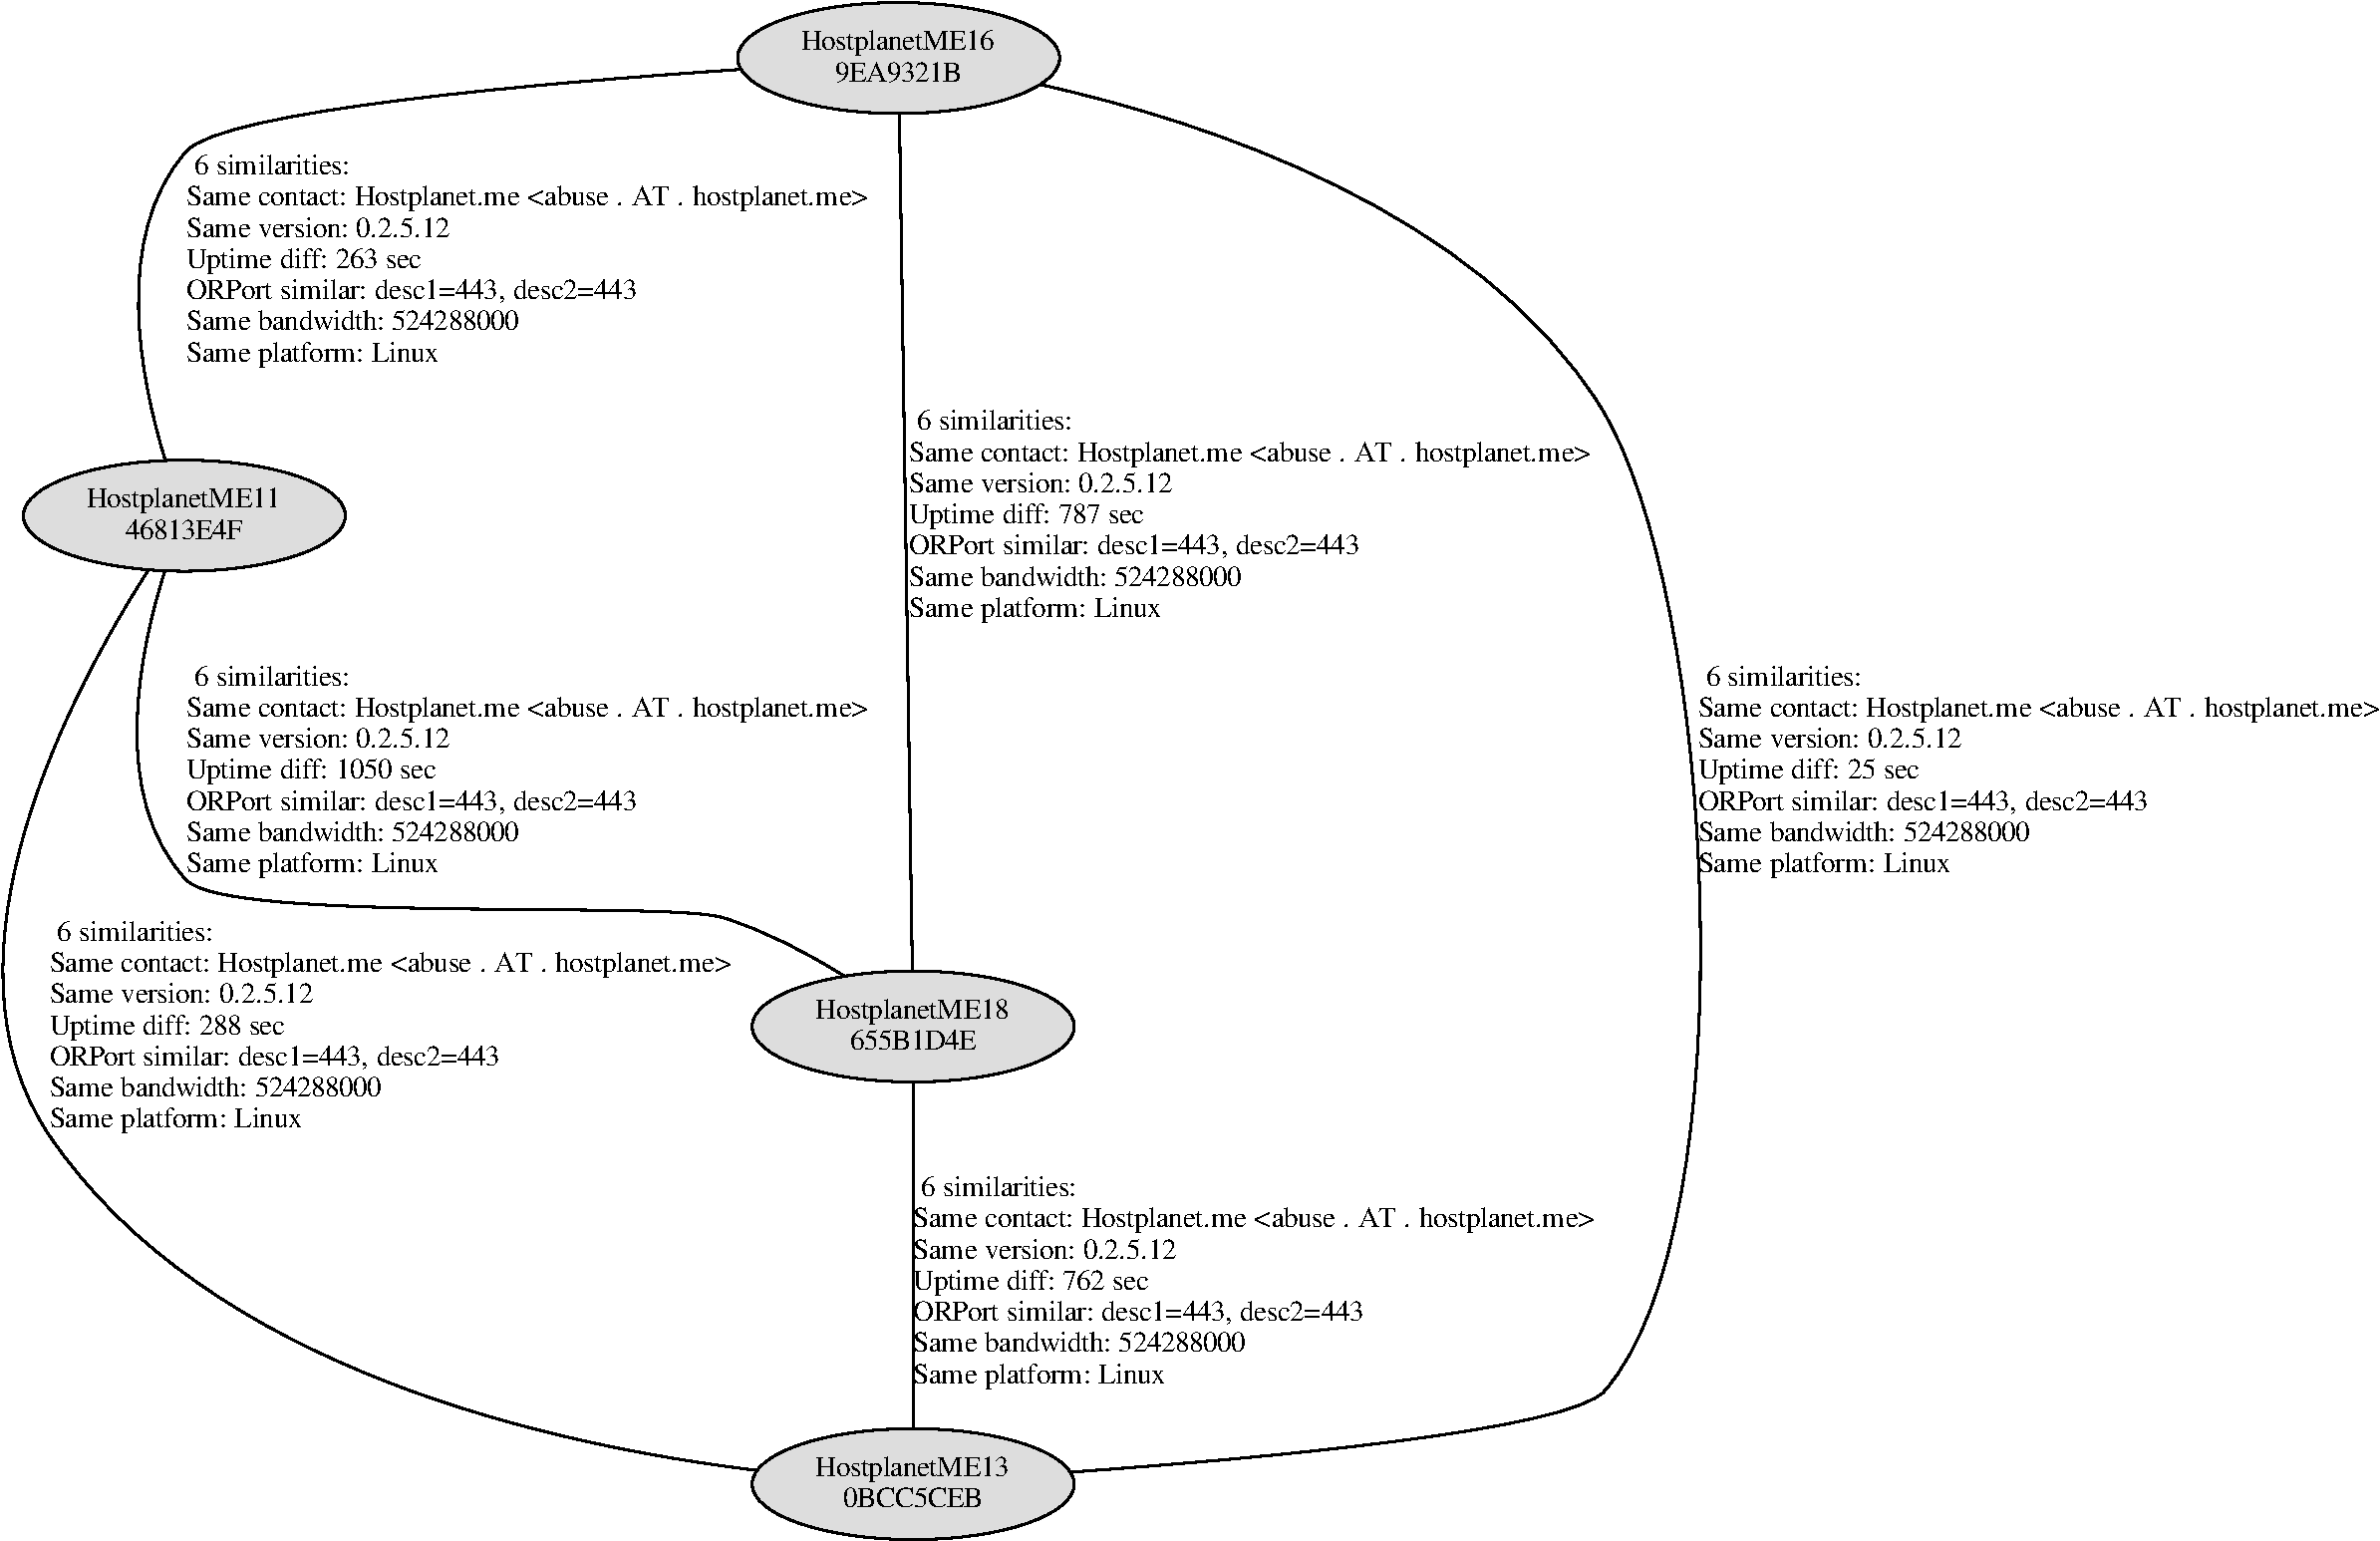
\includegraphics[width=0.42\textwidth]{diagrams/visualization.pdf}
    \caption{Visualization of a Sybil cluster.  Vertices represent Tor relays
    and edges show the similarities between them.}
	\label{fig:visualization}
\end{figure}
